\documentclass[aspectratio=169,11pt]{beamer}
\usepackage[T1]{fontenc}
\usepackage{lmodern,booktabs,array,tikz}
\definecolor{Ink}{HTML}{17324D}
\definecolor{Teal}{HTML}{007F7B}
\definecolor{Gray}{HTML}{657483}
\definecolor{Soft}{HTML}{EEF3F6}
\setbeamercolor{normal text}{fg=Ink,bg=white}
\setbeamercolor{frametitle}{fg=Ink}
\setbeamercolor{structure}{fg=Teal}
\setbeamercolor{block title}{fg=white,bg=Teal}
\setbeamercolor{block body}{fg=Ink,bg=Soft}
\setbeamertemplate{navigation symbols}{}
\setbeamersize{text margin left=9mm,text margin right=9mm}
\setbeamerfont{frametitle}{size=\large,series=\bfseries}
% Update this file only from a checked, paired evaluation.
% Keep the visible slide, speaker guide, evidence file, and notes in sync.
\newcommand{\EvidenceCutoff}{7 Oct 2026, 09:27 UTC}
\newcommand{\PilotBefore}{20}
\newcommand{\PilotAfter}{22}
\newcommand{\PilotTotal}{64}
\newcommand{\PilotNewCorrect}{3}
\newcommand{\PilotNewWrong}{1}
\newif\iffinalresults
\finalresultsfalse
\newcommand{\FinalBefore}{pending}
\newcommand{\FinalAfter}{pending}
\newcommand{\FinalTotal}{128}
\newcommand{\FinalNewCorrect}{pending}
\newcommand{\FinalNewWrong}{pending}
\newcommand{\FinalInterpretation}{One short run is preliminary; repeat before claiming a reliable gain.}

\setbeamertemplate{footline}{\hspace{9mm}\scriptsize Lessons from math RL for RLMs | \EvidenceCutoff\hfill\insertframenumber/\inserttotalframenumber\hspace{9mm}\vspace{3mm}}
\newcommand{\aside}[1]{\vfill{\footnotesize\color{Gray}#1\par}}
\hypersetup{pdftitle={Preparing language models to learn from practice},pdfauthor={Alex Towell}}
\begin{document}

\begin{frame}[t]
\frametitle{Before rewarding success, make success reachable.}
\textbf{Our goal:} Teach a recursive language model (RLM) to solve problems by using Python, asking helpers, and combining their results.
\medskip
\begin{block}{The question behind our experiments}
Why can reinforcement learning (RL) improve a math model, while our RLM training has struggled to produce reliable gains on new tasks?
\end{block}
\medskip
\textbf{Working explanation:} Math training builds on relevant prior competence. An RLM may need help applying familiar skills in an unfamiliar workflow.
\medskip

\textbf{Teaching implication:} Check what the learner can already do, teach the missing pieces, then give it useful practice and feedback.
\aside{RL learns from scored attempts. An RLM combines language-model calls with a code workspace. We are exploring what preparation makes this learning effective.}
\end{frame}

\begin{frame}[t]
\frametitle{Math RL builds on a strong head start.}
\textbf{Pretraining did much of the preparation:} our starting model had already learned from extensive mathematical text and worked solutions.
\medskip
\begin{columns}[T,onlytextwidth]
\begin{column}{0.52\textwidth}
{\small Correct final answers / same 64 MATH500 questions}
\begin{center}
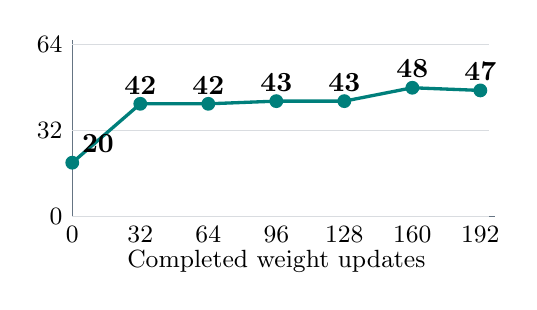
\begin{tikzpicture}[x=0.027cm,y=0.034cm]
\draw[Gray] (0,0)--(199,0);
\draw[Gray] (0,0)--(0,66);
\foreach \y in {0,32,64} {\draw[Gray!25] (0,\y)--(196,\y);\node[left,font=\small] at(0,\y){\y};}
\foreach \x in {0,32,64,96,128,160,192} {\node[below,font=\small] at(\x,0){\x};}
\draw[Teal,very thick] (0,20)--(32,42)--(64,42)--(96,43)--(128,43)--(160,48)--(192,47);
\fill[Teal] (0,20) circle(2.5pt);\node[above right,font=\normalsize\bfseries] at(0,20){20};
\foreach \x/\y in {32/42,64/42,96/43,128/43,160/48,192/47} {\fill[Teal] (\x,\y) circle(2.5pt);\node[above,font=\normalsize\bfseries] at(\x,\y){\y};}
\node[below,font=\small] at(96,-9){Completed weight updates};
\end{tikzpicture}
\end{center}
\end{column}
\begin{column}{0.44\textwidth}
\small
\textbf{Prior skill:} it can already solve some problems.
\medskip

\textbf{Exploration:} multiple attempts reveal successes and mistakes.
\medskip

\textbf{Feedback:} an answer checker distinguishes them, giving training something useful to reinforce.
\end{column}
\end{columns}
\aside{One greedy answer per question, fixed prompt and checker; repeatedly inspected development set. Small-scale improvement, not a full-benchmark replication. Prompt choice matters.}
\end{frame}

\begin{frame}[t]
\frametitle{An RLM must combine skills in a new setting.}
Knowing Python or answering questions does not guarantee knowing \textbf{our tool interface}, \textbf{what to delegate}, or \textbf{what a helper needs to know}.
\medskip
\begin{block}{Invented example: which city does Mira work in?}
One document says ``Mira works at Aster Lab.'' Another says ``Aster Lab is in Oxford.'' To find the city, the second helper needs \emph{Aster Lab}, not just ``find the city.''
\end{block}
\medskip
An attempt can fail through a bad call, missing context, a mistaken helper, or a bad plan. A final ``wrong'' score does not say which one to repair.

\medskip
\textbf{Our history:} some routines improved; reliable transfer to new combinations remained limited.
\aside{An unfamiliar workflow is a possible distribution shift, not a measured explanation of every earlier failure.}
\end{frame}

\begin{frame}[t]
\frametitle{Useful practice is challenging, but within reach.}
\textbf{Human analogy:} a child missing algebra needs more than a calculus test marked ``wrong.'' A simpler exercise and a worked example give a place to start.

\medskip
\textbf{Model example:} Solve $3x+2=14$. An attempt answering $x=4$ succeeds; one answering $x=5$ fails.
\smallskip
\begin{center}
\renewcommand{\arraystretch}{1.15}
\begin{tabular}{ll}
\toprule
Attempts on the same problem & What the reward comparison offers \\
\midrule
All wrong & No successful example to favor \\
Some right, some wrong & A contrast to learn from \\
All right & No distinction between attempts \\
\bottomrule
\end{tabular}
\end{center}
\textbf{Curriculum idea:} choose reachable challenges and increase difficulty as skills develop.
\aside{Human learning is an analogy. The reward comparison here is specific to our method; other kinds of RL can learn from other feedback.}
\end{frame}

\begin{frame}[t]
\frametitle{Teach, practise, remove help, then test transfer.}
\textbf{One possible approach, inspired by teaching:} watch a worked example, solve with hints, then solve a new problem independently.
\medskip
\begin{center}
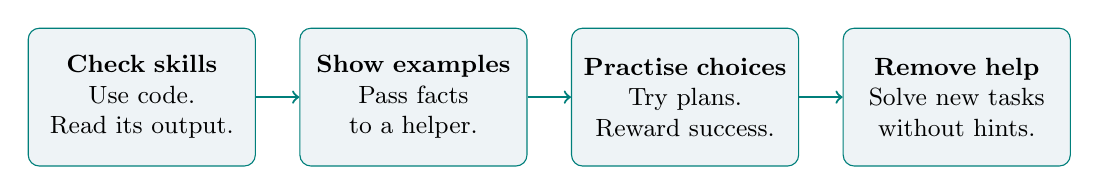
\begin{tikzpicture}
\tikzset{skill/.style={draw=Teal,fill=Soft,rounded corners,align=center,text width=2.65cm,minimum height=1.75cm,font=\small}}
\node[skill] (a) at(0,0) {\textbf{Check skills}\\Use code.\\Read its output.};
\node[skill] (b) at(3.45,0) {\textbf{Show examples}\\Pass facts\\to a helper.};
\node[skill] (c) at(6.90,0) {\textbf{Practise choices}\\Try plans.\\Reward success.};
\node[skill] (d) at(10.35,0) {\textbf{Remove help}\\Solve new tasks\\without hints.};
\draw[->,Teal,thick] (a)--(b);
\draw[->,Teal,thick] (b)--(c);
\draw[->,Teal,thick] (c)--(d);
\end{tikzpicture}
\end{center}
\medskip
\textbf{For the RLM:} first demonstrate passing an employer's name to a helper. Later, omit that hint and ask it to decide which facts and helpers it needs.
\medskip

\textbf{The real test:} can it use the skills in a new situation, rather than repeat a taught routine?
\aside{One hypothesis to test. Examples can be shown in a prompt or learned through supervised fine-tuning (SFT). Teach missing skills, not everything from scratch.}
\end{frame}

\begin{frame}[t]
\frametitle{Different failures need different interventions.}
\begin{block}{It cannot produce a successful attempt}
Clarify the interface, show a verified example, simplify the task, or try a more capable starting model. More retries alone may repeat the same failure.
\end{block}
\begin{block}{It succeeds occasionally}
More attempts or more varied plans may expose successes that RL can reinforce. Higher sampling temperature can add variety, but also invalid calls.
\end{block}
\begin{block}{It has successes and failures, but does not improve}
Check the feedback and weight updates. Does the score reward actual success? Can training identify which earlier decisions helped?
\end{block}
\aside{Possible remedies, not established diagnoses. More attempts cost compute; more randomness is not necessarily more useful exploration.}
\end{frame}

\begin{frame}[t]
\frametitle{An open agenda of small experiments.}
\textbf{We are exploring, not choosing a final recipe.} These are examples of questions we can test, not an exhaustive plan.
\medskip
\begin{center}
\renewcommand{\arraystretch}{1.2}
\begin{tabular}{p{0.30\textwidth}p{0.61\textwidth}}
\toprule
Possible explanation & Small comparison \\
\midrule
Ability is hidden & Same weights; clearer prompt or tool example. \\
A skill is missing & Teach one verified helper routine; test a new case. \\
Teaching order matters & Same examples and budget; staged vs. shuffled. \\
Successes are too rare & Vary attempts or plans; keep total cost comparable. \\
\bottomrule
\end{tabular}
\end{center}
\medskip
\textbf{For each:} measure after preparation, then after RL. Remove hints and test new combinations. Preparation working is not yet evidence that RL helped.
\aside{Other possibilities: error-and-repair examples, stronger starting models, better feedback, and different helper roles. Change one factor; use what we learn to refine, expand or retire ideas.}
\end{frame}
\end{document}
